\section{\label{sec:LaTeX}\LaTeX}

\ptitle{Intro to \LaTeX} \LaTeX\ is a formatting language that allows professional, publication-quality presentation of scientific text, equations, figures, and hyperlinked references. REVTeX is a specific set of \LaTeX\ macro packages assembled by the American Physical Society (APS) to standardize manuscript formatting for the various Physical Review journals. The APS author website \cite{PhysicalReview} lists acceptable submission formats as: REVTeX \textbf{(preferred)}, \LaTeX, or MSWord. It is sensible to draft your paper in \LaTeX/REVTeX from the beginning. You will need a reference manager, a text editor, and a \LaTeX\ compiler. Typically, you will be working closely with other authors, so you should pick a platform that enables simple sharing and collaborative workflow.

\ptitle{Overleaf} Here we recommend the online \LaTeX\ compiler Overleaf (\url{http://www.overleaf.com/}) for text editing and compiling. Overleaf (formerly known as Share\LaTeX) is an online platform that is great for collaborative writing: it tracks changes and even has a real-time chat function. Note that LyX is a WYSIWYG (what you see is what you get) \LaTeX\ editor that may seem tempting if you initially find tex formatting daunting, but LyX may come back to bite you in the long run, because it hides the guts of the tex code from the user, making it harder to control formatting details.

\begin{raggedright}
\begin{enumerate}
\item Choose \& install a reference management software such as Mendeley:
\url{http://www.mendeley.com/}\\
(See appendix \ref{app:Mendeley} for usage tips.)
\item Make an account on Overleaf:
\url{http://www.overleaf.com/}\\
\item Download the source files for this example paper:
\url{http://hoffman.physics.harvard.edu/example-paper/}
\item Copy the tex and bib files into a new overleaf project, and share with your collaborators.
\end{enumerate}
\end{raggedright}
\vspace{2mm}

\ptitle{Alternatives} Alternatively, you may prefer to run \LaTeX\ directly on your own laptop. In that case, follow the steps below:
\begin{raggedright}
\begin{enumerate}
\item Choose \& install a reference management software:
\begin{itemize}
\item Mendeley: \url{http://www.mendeley.com/}
\item Papers: \url{http://www.papersapp.com/}
\item Endnote: \url{http://www.endnote.com/}
\end{itemize}
\item Download \& install a \LaTeX\ compiler such as MikTex: \\
\url{http://miktex.org/}
\item Download \& install REVTeX 4-2 (see appendix \ref{app:REVTeX}):\\
\url{http://authors.aps.org/revtex4/}
\item Pick an editor such as WinEdt:
\url{http://www.winedt.com/}\\
(You may need to request a university license; may require $\sim 24$ hour turnaround.)
\item Download the source files for this example paper:
\url{http://hoffman.physics.harvard.edu/example-paper/}, open the tex and bib files in WinEdt, and get started writing!
\end{enumerate}
\end{raggedright}
\vspace{2mm}

\ptitle{Maintain your outline} It's important not to lose sight of your outline, as you fill in the details of your paper. This \LaTeX\ template file allows you to title each paragraph using the {\tt \textbackslash ptitle\{\}} command. You should keep these titles in place throughout the entire paper-writing process; they will serve as a constant reminder to keep each paragraph focused on a single point. You should be able to skim through these bold paragraph titles, without reading any of the intervening sentences, and still understand the basic logical flow of the paper. At the final step before submission, comment out the line {\tt \textbackslash ptitletrue} in the header, to hide the paragraph titles. But do not delete the paragraph titles, because they will remain useful to you in the inevitable paper revision process down the road!

% \section{Auswertung}
% \label{sec:Auswertung}
% %Fehlerrechnung
% Für die Auswertung der Messergebnisse wird im Folgenden der Mittelwert immer als
% \begin{equation}
%   \bar{x} = \frac{1}{N}\sum_{i=1}^{N} x_{i}
% \end{equation}
% berechnet und die Standardabweichung mit
% \begin{equation}
%   \Delta\bar{x} = \frac{\sigma}{\sqrt{N}} = \sqrt{\frac{1}{N(N-1)}\sum_{i=1}^{N} (x_{i} - \bar{x})^2}.
% \end{equation}
% Weiterhin wird die Gaußsche Fehlerfortpflanzung
% \begin{equation}
%   \Delta f = \sqrt{\left(\frac{\partial f}{\partial x}\Delta x\right)^2 + \left(\frac{\partial f}{\partial y}\Delta y\right)^2 + \dots}
% \end{equation}
% verwendet. Für Plots und Regression wird Python genutzt.
% %------------

% %Figur einbinden
% \begin{figure}
%   \centering
%   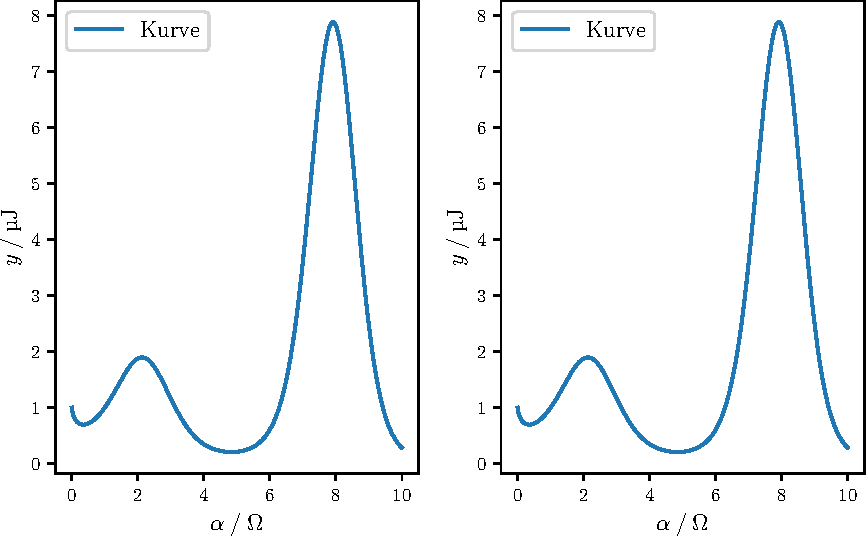
\includegraphics{plots/plot.pdf}
%   \caption{Plot.}
%   \label{fig:plot}
% \end{figure}
% %------

% %Tabelle einbinden
% \begin{table}
%   \centering
%   \caption{Beschreibung}
%   \label{tab:Beispiel}
%   \begin{tabular}{S[table-format=2.0] S[table-format=2.2]}
%     \toprule
%     {$f \:/\: \si{\kilo\hertz}$} & {$U_C \:/\: \si{\volt}$}\\
%     \midrule
% 50  & 4.08\\
% 52  & 3.76\\
%   \end{tabular}
% \end{table}
